\chapter{Implementation}
In this chapter the implementation of the language and the tool, the problems faced, and the solutions adopted will be discussed

\section{General overview of the tool}
\begin{figure}
    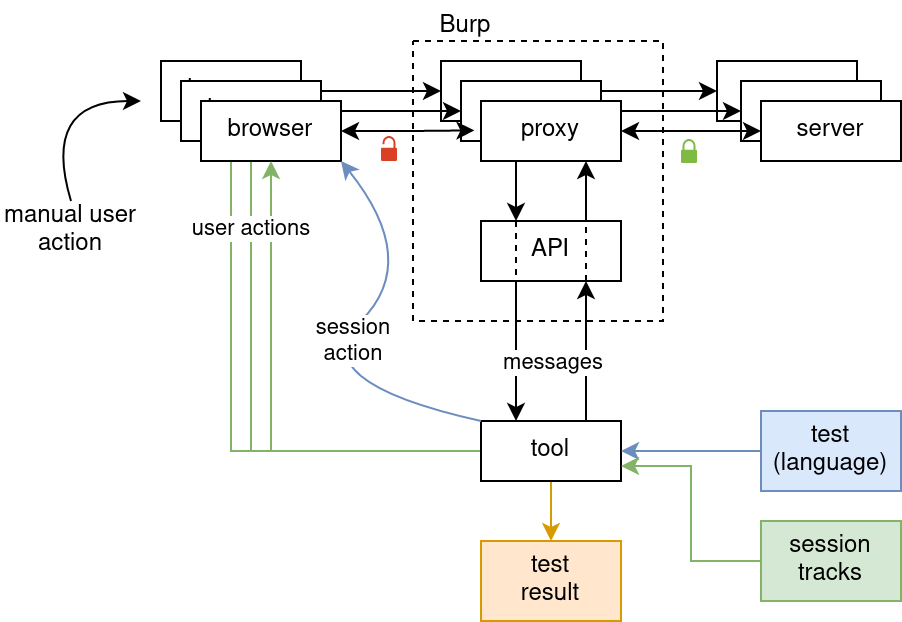
\includegraphics[width=\textwidth]{general_schema.png}
    \caption{General schema}
    \label{fig:general_schema}
\end{figure}

All the components of the final tool can be seen in \ref{fig:general_schema}. Burp Suite is composed by its proxy and related APIs, the tool will get all the messages from the proxy through the API, and then, it will return them to the API and so, to the proxy. This way all the messages will pass through the tool, and will make possible to make checks and edit them.
Every browser, (one for each session) will be using a dedicated proxy, which will act like a Man In The Middle attack from the browser to the server, establishing a secure connection only on the last part of the communication to the server, making possible to see plain HTTP communications on the browser side. Each browser will be supplied with the user actions which will be taken from the session tracks specified beforehand. It is also possible to do manual user actions on the browser, in case (for example) a captcha has to be resolved. Also, the session actions taken from the tests defined by the language can be supplied to the browser (for example to pause or stop it). The most important component of the tool is the Test Suite defined with the language, which is supplied to the plugin, and executed in ensemble with the sessions, giving eventually a result.

\section{The tool}
For the implementation of the \Gls{burp}'s tool introduced earlier, I have decided to start from a work done by my colleague Wendy Barreto in her bachelor thesis \cite{wendy_barreto}, which realized a similar tool for \Gls{OIDC} and \Gls{OAuth} SSO protocols, this was a good base to start with my implementation. The interface of \cite{wendy_barreto} has been taken and adapted to fit the needs of this work. The tool code is written in Java, I used the \Gls{burp}'s interface classes to interact with it.
The standard usage of \Gls{burp} is based on the execution of a browser which connects to the \Gls{burp}'s proxy, in a way that all the packets can be intercepted, viewed or edited and forwarded or dropped from the \Gls{burp} interface. The tester would do some actions on the browser and watch the flowing packets in \Gls{burp} and then check them or edit them. With the tool the idea is the same, but the operation done on the browser and the checks or edits on the messages are made automatically, in a way that the tester doesn't have to do them by itself.

\begin{figure}
    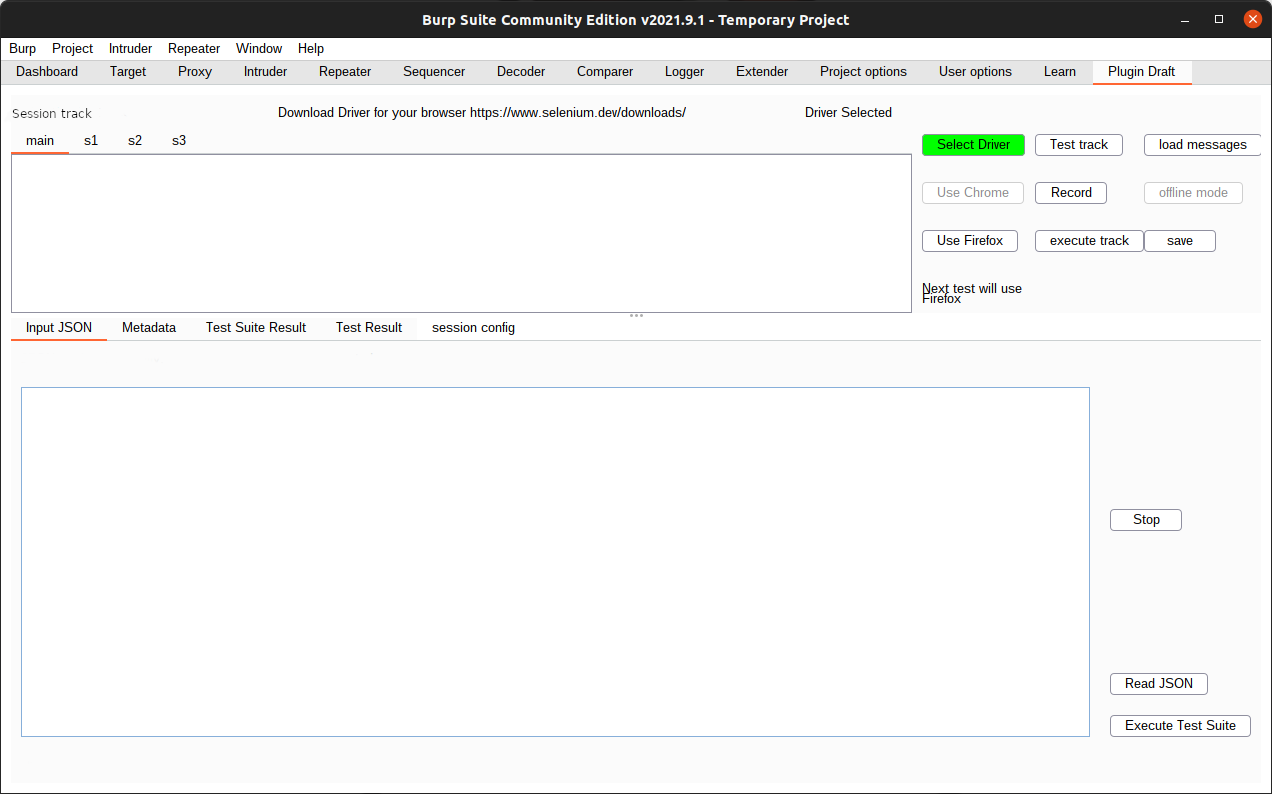
\includegraphics[width=\textwidth]{interface.png}
    \caption{Tool interface}
    \label{fig:plugin_interface}
\end{figure}

\subsection{Interface of the tool}
In figure \ref{fig:plugin_interface} we can see the interface of the tool, starting from top left we have the session track input space, where it can be specified a different track for each session. Following on the top right, wee have a series of buttons that allow various configurations:
\begin{itemize}
    \item the browser to be used can be selected
    \item the driver to automate the actions on the browser can be selected
    \item the record button can be used to record the passing messages
    \item the load messages button can be used to load the previously saved messages to be tested "offline"
    \item the offline mode button to test the loaded messages instead of the live ones
\end{itemize}

In the bottom part we have multiple tabs:
\begin{itemize}
    \item "Input JSON" tab is used to load the tests written in the language into the tool, and with the use of two buttons we can parse the language and execute the tests.
    \item "Test suite result" is the tab containing all the results of the executed tests
    \item "Test result" is the tab used to see the specific test result, with all the intercepted messages related to it
    \item "Session config" is used to configure the ports of the sessions that will be used in the tests.
\end{itemize}

\subsection{Test execution}
The test execution differs from passive to active, as passive tests do not need the edit of the messages, the execution of the \gls{session track} is done once, the messages are saved and the tests are executed on the saved messages. I have also added the possibility of exporting the saved messages to a file, in a way that they can be imported in the tool and tested again.
On the other hand, active tests needs to edit the messages, so the execution of the track has to be repeated for each test.

\subsection{Decoding \& encoding of parameters}
As said in the previous chapter, the decoding and encoding of parameters is possible. To do that, a list of encodings to be done on the parameter has to be provided, i.e. url, base64, deflate. Once the specified message is intercepted, the parameter is taken and decoded following the order of the provided encodings list. To do that, part of the code of SAML Raider \cite{saml_raider} which did the decoding of \Gls{SAML} Requests and responses parameters has been used. That part of the code has been taken and edited to fit the tool. SAML Raider is a \Gls{burp}'s plugin used to manage \Gls{SAML} certificates.

\subsection{SAML certificate managing}
In \Gls{SAML} Requests and responses there is sometime the need to remove or edit the certificate associated to that request or response, so, to speed up the process a specific tag in the language has been added to remove or edit the certificate signature. There is still the possibility of doing the same removal by editing the \Gls{SAML} request or response with a regex, but with the use of the tag this becomes more convenient.
In order to do this, a part of the code of SAML Raider \cite{saml_raider} has been used, edited to fit the needs.

%
%\subsection{Oracle}
%To identify abnormal pages like error pages the \gls{session track} evaluation should be sufficient, because if some actions could not be executed means that the original "flow" of pages was not followed.

\subsection{Session managing}
The sessions are managed independently, each session is basically a browser that is launched when a session is started. Each session can follow a different \gls{session track} defined in the apposite tabs. Every session is run in a separated thread to make parallelism possible. By the use of specific commands in the language, is possible to do some actions on each session, like stop it, pause it, or clear its cookies. Each browser uses a different proxy port, so that it is possible to know from which session the messages come from, and so, being able to specific sessions in the tests.







